\chapter{Utvärdering av befintliga verktyg}
\label{sec:forarbete}
För att förstå hur systemet skulle utvecklas, och om det redan fanns liknande lösningar utvärderades alla kända implementationer som berörde liknande ämnesområden som det här arbetet. Implementationerna presenterades i kapitel \ref{sec:teori:schema-användningsområden} och kommer diskuteras mer djupgående i detta kapitel. Resultatet från utvärderingen av verktyg som genererar eller parsar JSON Scheman var att inget verktyg passade användningsområdet, och att en implementation var trivial. Därför beslutades det att både generering och parsning implementeras skulle skapas av författaren. Samtliga verktyg som genererar grafiska användargränssnitt utifrån JSON Scheman var anpassade för hemsidor \textit{(HTML, CSS och JavaScript)}, vilket hindrade verktygen från att integreras med systemet som skrevs i Delphi som en skrivbordapplikation till Windows. Därför fick även det verktyget skapas av författaren.

\section{Implementationer som utesluts ur rapporten}
Vissa av implementationerna uteslöts från rapporten då det ansågs vara omöjligt att förstå implementationerna. \textit{Schema Guru Web UI} kunde inte hittas. \textit{AutoParse} är ett verktyg som inte uppdaterats sedan 26 Mars 2013, vilket betyder att den som bäst kan implementera version tre av JSON Schema \cite{Googleb}. Dessutom länkar projektet till en hemsida som länkar tillbaka till projektet, vilket saknar dokumentation \cite{Googleb}. Verktyget \textit{gojsonschema} saknade tillräcklig information på engelska eller svenska \cite{Zhangtao}. \textit{Jsonary} hade bristande dokumentation, med länkar till en hemsida som inte finns \cite{Jsonary-js}. Länken till \textit{pure-form webcomponent} på Json Schemas hemsida returnerade felkoden 404 vilket betecknar att webbsidan som efterfrågats inte finns eller inte kan hittas. Efter omfattande sökningar hittades inte verktyget.

\section{Generering av scheman från JSON}
\label{sec:forarbete:json-till-schema}
Att generera JSON Scheman från en JSON-fil perfekt, är omöjligt. Att bara observera en JSON-fil tillför inte tillräcklig infomation för att generera ett JSON Schema. Studera exemplet i figur \ref{fig:json-super-simple-example}. Att skapa ett JSON Schema som beskriver det objektet skulle kunna se ut som i figur \ref{fig:schema-super-simple-example-1}. Då har antaganden tagits om att det objektet alltid ska ha en \textit{property} som heter \textit{name} och ska innehålla en textsträng. Det skulle kunna vara så att \textit{name} alltid ska innehålla en textsträng som börjar på stor bokstav, vilket är rimligt när det representerar ett namn, och då skulle schemat se ut som i figur \ref{fig:schema-super-simple-example-2}. Det skulle annars kunna vara så att \textit{name} inte får vara vilken textsträng som helst utan måste vara en av två textsträngar. Det skulle till och med kunna vara så att \textit{name} också skulle kunna vara det booleska värdet \textit{false}. Då skulle schemat se ut som i figur \ref{fig:schema-super-simple-example-3}.

\begin{figure}
	\inputminted[tabsize=2, frame=single, fontsize=\small, framesep=2mm]{json}{code/schema-generation-example/json-file.json}
	\vspace{-1.7em}
	\caption{Exempel på enkelt JSON-objekt}
	\label{fig:json-super-simple-example}
\end{figure}

Alla de här exemplen har enbart behandlat feltolkning av en \textit{property} och inte diskuterat ännu större missförstånd med objektets struktur. Objektet skulle möjligtvis kunna ha en valfri \textit{property} som representerar efternamn. Då skulle schemat se ut som i figur \ref{fig:schema-super-simple-example-4}. Alla exempel är giltiga scheman till objektet i det givna exemplet. Det finns ingen möjlighet att förstå vilket schema som faktiskt beskriver datan, utan att göra många antaganden om datan. Därför ansågs samtliga lösningar som genererar JSON Scheman från JSON-filer vara otillräckliga för projektet.

\begin{figure}
	\begin{subfigure}[t]{0.47\textwidth}
		\inputminted[tabsize=2, frame=single, fontsize=\small, framesep=2mm]{json}{code/schema-generation-example/schema-example1.json}
		\vspace{-1.2em}
		\caption{Exempel på genererat schema}
		\label{fig:schema-super-simple-example-1}
	\end{subfigure}\hfill
	\begin{subfigure}[t]{0.47\textwidth}
		\inputminted[tabsize=2, frame=single, fontsize=\small, framesep=2mm]{json}{code/schema-generation-example/schema-example2.json}
		\vspace{-1.2em}
		\caption{Exempel på genererat schema med strängmönster}
		\label{fig:schema-super-simple-example-2}
		\vspace{.8em}
	\end{subfigure}
	\begin{subfigure}[t]{0.47\textwidth}
		\inputminted[tabsize=2, frame=single, fontsize=\small, framesep=2mm]{json}{code/schema-generation-example/schema-example3.json}
		\vspace{-1.2em}
		\caption{Exempel på genererat schema med \textit{enums}}
		\label{fig:schema-super-simple-example-3}
	\end{subfigure}\hfill
	\begin{subfigure}[t]{0.47\textwidth}
		\inputminted[tabsize=2, frame=single, fontsize=\small, framesep=2mm]{json}{code/schema-generation-example/schema-example4.json}
		\vspace{-1.2em}
		\caption{Exempel på genererat schema med dolda \textit{properties}}
		\label{fig:schema-super-simple-example-4}
	\end{subfigure}
	\caption{Olika JSON Scheman som är kompatibla med JSON-objektet i figur \ref{fig:json-super-simple-example}}
	\label{fig:schema-super-simple-example-group}
\end{figure}

\section{Generering av scheman från statiska datatyper i statiskt typade programmeringsspråk}
Det finns implementationer som utnyttjar att statiskt typade programmeringsspråk redan innehåller beskrivningar av data som ska bearbetas. Både .Net och TypeScript erbjuder programmeringsfunktioner inbyggda i språket för att beskriva komplexa datastrukturer. Att sedan översätta dem till JSON Schema-filer presterar riktigt bra. Varken .Net eller TypeScript erbjuder stöd för att exempelvis bestämma att ett tal bara får befinna sig inom ett bestämt intervall, och det saknas fler specificiteter som JSON Schema erbjuder. För att bemöta de bristerna använder samtliga implementationer speciellt formaterade kommentarer som kallas annotationer, vilket möjliggör all funktionalitet som JSON Schema erbjuder. Att TypeScript är ett språk som kompileras till JavaScript, vilket JSON och i sin tur JSON Scheman bygger på innebär att översättningen mellan datatyper i TypeScript och JSON Scheman resulterar i väldigt korrekta resultat. \cite{Newtonsoft,Suter,El-Dardiry,Bovet}

Implementationer skrivna för .Net eller TypeScript ansågs vara svåra och möjligtvis omöjliga att integrera i systemet. Det är självklart en subjektiv bedömning tagen av författaren. Bedömningen baseras på att all kod som hanterar JSON Scheman måste vara skrivet i antingen plattformen .Net eller språket TypeScript. Det skulle innebära att en stor del av systemet vore skrivet i ett språk som inte är Delphi, samt att de två delarna av systemet skulle behöva integreras. Då generering av JSON Schema är relativt trivialt ansågs det vara enklare och mer långsiktigt att skapa ett eget verktyg.

\section{Andra genererare av scheman}
\textit{Liform} och \textit{JSL} erbjuder metoder och funktioner som underlättar dynamiskt skapande av JSON Scheman under exekvering. De erbjuder datatyper som är inbyggda i språket för att definiera och hantera komponenter av JSON Scheman. De kan sedan generera ett JSON Schema utifrån de här instanserna av datatyperna. \cite{Romanovich,Limenius}

\textit{Liform} ansågs vara väldigt enkelt att använda och passade användningsområdet. Det använder dessutom den senaste standarden av JSON Schema. Däremot är \textit{Liform} skrivet i och för språket PHP, vilket inte är kompatibelt med Delphi. Därför ansågs inte \textit{Liform} vara enkelt att integrera med resten av systemet.

\textit{JSL} ansågs också passa användningsområdet men använde inte den senaste standarden av JSON Schema. Dessutom var \textit{JSL} skrivet i och för språket Python vilket inte är kompatibelt med Delphi.

\textit{APIAddIn} är ett plugin åt \textit{Sparx Enterprise Architect}, vilket är ett verktyg för modellering, visualisering och design av system, mjukvara, processer eller arkitekturer. Verktyget baseras på UML vilket är ett generellt språk för modellering av system. Det erbjuder delvis en liknande funktion som JSON Schema erbjuder. Om datan som skulle beskrivas av JSON Scheman redan fanns definierade med UML, skulle det möjligtvis vara ett rimligt alternativ att överväga, men då datan inte fanns definierat med UML ansågs APIAddIn vara ett onödigt verktyg, när schemat lika gärna kan definieras med JSON Schema från första början. \cite{Tomlinson}

Online-verktyget \textit{JSONSchema.net} är ett verktyg för att skapa JSON Scheman, med hjälp av ett grafiskt användargränssnitt. Det erbjöd inte mer funktionalitet än att skriva JSON Schemat manuellt. Dessutom genererade den inte JSON Scheman enligt den senaste standarden. \cite{Jackwootton}

\section{Parsning av JSON Scheman}

En viktig del i all hantering av JSON Scheman är självklart parsningen, vilket är utförandet av att läsa och tolka JSON Schemat, för att sedan representera innehållet på nytt med en annan representation som är mer användbar för syftet. Vissa parsers tolkar ett JSON Schema, och genererar kod för att hantera JSON-filer som är strukturerade efter det schemat. Det kan också användas för att programmet dynamiskt ska förstå hur en JSON-fil ska läsas. Dessutom kan det handla om att parsa ett JSON Schema för att skapa ett dynamiskt test för att testa om given JSON-data är korrekt formaterad, utifrån det givna schemat.

\textit{DJsonSchema} är ett verktyg som parsar ett JSON Schema och sedan genererar kod som klarar av att parsa JSON som följer samma struktur som schemat. DJsonSchema är skrivet i Delphi och genererar kod för Delphi, vilket är samma språk som konfigurationssystemet skrevs i. Systemet krävde dynamisk parsning av scheman så därför passar inte DJsonSchema för parsning i detta projekt. Utöver det saknades stöd för version sju av JSON Schema. DJsonSchema uppger dessutom att implementationen var ofullständig. \cite{Schlothauer&WauerGmbH}

\textit{jsonCodeGen} hade bristfällig dokumentation. Det framstod att det var ett verktyg som parsar en utökad version av JSON Scheman som inte var kompatibel med den senaste officiella, eller någon tidigare officiell JSON Schema specifikation. Dessutom var verktyget skrivet för Groovy, vilket också gör den kompatibel med Java, men inte Delphi. Utifrån beskrivningen av hur verktyget skulle användas framstod det som att verktyget genererar statiska filer utifrån JSON Scheman eller JSON-filer, vilket inte är dynamiskt som konfigurationssystemet kräver. Det är också värt att nämna att utvecklarna av jsonCodeGen är samma utvecklare som utvecklade DJsonSchema. \cite{Schlothauer&WauerGmbHa} 

\textit{aeson-schema} är ett verktyg för att validera ett JSON-värde mot ett schema, eller för att generera en JSON parser åt JSON-filer som är strukturerade efter ett givet schema. Det garanterar att om ett JSON-värde blivit godkänd i validering, kan samma JSON-värde parsas och användas i ett program skrivet i Haskell. Verktyget implementerar version tre av JSON Schema, vilket inte är version sju som projektet använder. \cite{Kowalczyk}

\textit{json-schema-codegen} stöder stora delar av JSON Schema men inte allt. Verktyget parsar ett JSON Schema och genererar sedan kod som kan parsa JSON som är strukturerade efter schemat. \cite{Tundra}

\textit{Argus} är ett verktyg som erbjuder nästan exakt den funktionalitet arbetet skulle implementera, vilket var att dynamiskt parsa JSON Scheman och sedan erbjuda en JSON parser som parsar JSON-filer som har strukturen som är beskriven av schemat. Parsern som parsar JSON-filerna kunde sedan erbjuda representationer av datan i form av datastrukturer som är kompatibla med programmeringsspråket programmet är skrivet i. Argus implementerades i Scala, vilket inte är kompatibelt med Delphi. \cite{Fenton} \textit{Bric-à-brac} är också ett verktyg som liknade Argus i funktionalitet, fast implementerat i språket Swift \cite{GlimpseI/OInc}. En notering är att dokumentationen är motstridig då den påstår att verktyget erbjuder en oföränderlig \textit{immutable} datastruktur, men den i exempelkoden visar motsatsen \cite{GlimpseI/OInc}. Det skulle kunna vara en indikator för att projektet inte är helt felfritt.

\textit{jsonschema} är ett verktyg som dynamiskt parsar JSON Scheman och erbjuder en instans som kan användas för att validera JSON-filer. Projektet är skrivet i Golang, vilket inte är kompatibelt med Delphi. \cite{Qriinc.}

Många av dessa projekt saknar tillräcklig dokumentation, vilket gör det omöjligt att använda dem i ett projekt. Dessutom är parsningen av JSON Scheman relativt enkelt, då det enbart handlar om att parsa JSON-filer som följer en förutbestämd struktur. Dessutom skiljer sig användningsområdena sig starkt efteråt, vilket kan kräva unik anpassning av JSON Schema-parsern, vilket är en stor anledning till att det finns så många olika sorters parsers. Ett annat problem att ta hänsyn till med implementationerna är att många av dem bara erbjuder generering av statisk kod i förväg, och klarar inte av att tolka olika JSON Scheman under exekvering av programmet. Det här arbetet handlar om att dynamiskt tolka olika sorters scheman för att anpassa ett användargränssnitt till servern som klienten kommunicerar mot, vilket innebär att de implementationerna är oanvändbara. Det sista och största problemet med implementationerna är att bara en var kompatibel med Delphi, vilket är språket som systemet skrevs i, och det ansågs vara otillräckligt. Med hänvisning till att det är relativs enkelt att skriva en parser och med problematiken alla implementationer presenterade, skrevs en egen parser åt det här arbetet.

\section{Användargränssnitt genererade baserat på JSON Scheman}
\label{sec:forarbete:gui-generering}
Samtliga implementationer som genererar grafiska användargränssnitt utifrån JSON Scheman, gör det för hemsidor \textit{(HTML, CSS och JavaScript)}. Att generera ett grafiskt användargränssnitt, baserat på JSON Scheman, med ett annat språk än JavaScript kan presentera hinder eller svårigheter. Att använda ett webbaserat grafiskt användargränssnitt var inte ett alternativ för systemet men samtliga implementationer undersöktes, för att ta lärdom om hur de fungerade. Många lösningar separerar JSON Schemat med datan som JSON Schemat beskriver. Den faktiska datan som det grafiska användargränssnittet visar, och sedan manipulerar kommer också kallas modell i resten av rapporten.

Att använda JSON Schema för att generera grafiska användargränssnitt kan ske på olika sätt, och många implementationer bygger på att ytterligare information tillförs för att kunna specificera hur modellerna ska representeras i det grafiska användargränssnittet. Vissa lösningar är generella för användning på vilken hemsida som helst, medan andra är kopplade till att användas med ett visst ramverk, som React, JQuery eller Angular.

\newpage

Alpaca Forms är en unik lösning då den är den enda implementationen som inte använder ett JSON Schema som är formaterat med JSON, utan schemat är en instans av ett JavaScript-objekt, vilket möjliggör att schemat inkluderar funktionslogik; En funktionalitet som saknas hos JSON. Utöver funktionslogik, inkluderar schemat en \textit{property} som kallas \textit{options}, som används för att beskriva hur det grafiska användargränssnittet ska se ut. De delarna av schemat som är korrekt JSON Schema används till stor del enbart för att koppla ihop det grafiska användargränssnittet med datan. \cite{GitanaSoftwareInc.}

Andra lösningar som utökade det officiella JSON Schemat är:
\begin{itemize}
	\item Angular2 Schema Form \cite{MakinaCorpus}
	\item JSON Editor \cite{JeremyDorn}
	\item json-forms \cite{Brutusin.org}
	\item JSONForms \cite{EclipseSource}
	\item liform-react \cite{NachoMartin}
	\item Metawidget \cite{Metawidget}
	\item React JSON Schema Form \cite{MozillaServices}
\end{itemize}

En annan lösning till problemet är att använda ett separat JSON-objekt som fungerar som ett schema för formulärets utseende och beteende. Lösningarna som använder den sortens lösning är:
\begin{itemize}
	\item Angular Schema Form \cite{Textalk}
	\item Angular2 Schema Form \cite{MakinaCorpus}
	\item JSON Form \cite{Joshfire}
	\item json-forms \cite{Brutusin.org}
	\item JSONForms \cite{EclipseSource}
	\item liform-react \cite{NachoMartin}
	\item React JSON Schema Form \cite{MozillaServices}
	\item React Schema Form \cite{NetworkNewTechnologiesInc.}
\end{itemize}

Observera att vissa implementationer både utökar JSON Schemat, och lägger till extra scheman för att beskriva formulärets utseende och beteende. Vissa lösningar utökar schemat för att sedan lägga till ett extra mellansteg där vissa parametrar i modellen kopplas till extra funktionslogik. Inget verktyg ansågs vara enkelt att integrera med systemet då de skrevs för att fungera med hemsidor. Dessutom skrevs många verktyg för fel version av JSON Schema. Utöver det så använde nästan alla verktyg ett externt \textit{``ui-schema''} eller inkompatibla JSON Scheman. Därför ansågs inga verktyg vara tillräckliga och ett nytt skapades.

\section{Fördjupad utvärdering av grafiska användargränssnitt baserade på JSON Scheman}
\label{sec:forarbete:kategorisering}

De grafiska användargränssnitt som genererades av verktygen går att dela in i två kategorier vilket här kallas \textit{trädstruktur} samt \textit{platt formulär}. En \textit{trädstruktur} är ett grafiskt användargränssnitt som erbjuder en generell JSON-editor där datan visuellt representeras med en trädstruktur. Det finns många exempel på grafiska användargränssnitt som erbjuder ett grundläggande gränssnitt för att redigera generell JSON-data. De skiljer sig inte mycket mot att skriva JSON manuellt, men kan erbjuda enkel hjälp med nyckelord och formatering. Figur \ref{fig:json-editor} visar JSON Editor Online, vilket är ett exempel på ett sådant grafiskt användargränssnitt \cite{DeJong2018}. Det skulle kunna gå att begränsa vad användaren skulle kunna mata in med hjälp av JSON Schemat men ett sådant formulär har möjlighet att hantera JSON Data som följer all möjlig sorts struktur.

En stor fördel med \textit{trädstrukturer} är att då de speglar strukturen av ett JSON-dokument kan de enkelt användas för att visualisera nästan vilken sorts JSON-data som helst, oberoende datans komplexitet. En nackdel med att använda ett sådant grafiskt användargränssnitt är att det inte är enkla att anpassa för ändamålet, och det grafiska användargränssnittet blir inte särskilt frikopplat mot datan som ska manipuleras. Det blir dessutom svårt att presentera information till användaren som kan hjälpa användaren förstå hur datan kommer användas.

\begin{figure}
	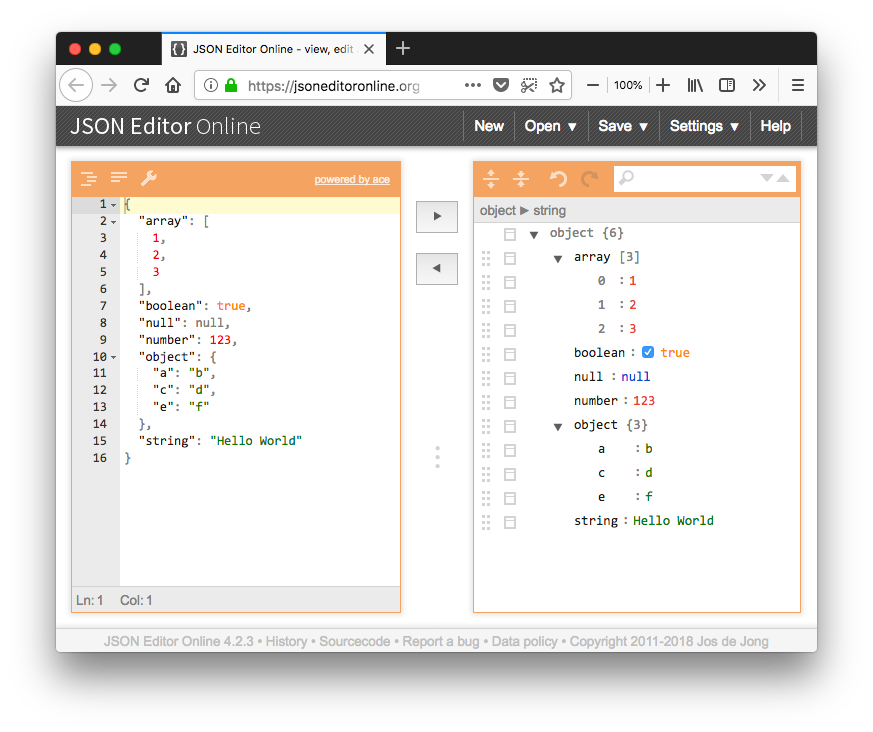
\includegraphics[width=\textwidth]{./images/screenshot-json-editor.png}
	\vspace{-1.7em}
	\caption{JSON Editor Online \cite{DeJong2018}}
	\label{fig:json-editor}
\end{figure}

Ett annat alternativ är att göra som React JSON Schema Form (se figur \ref{fig:react-jsonschema-form}), vilket då hamnar i kategorin \textit{platt formulär}. React JSON Schema Form genererar ett webbformulär utifrån ett JSON Schema och ett extra JSON-dokument som kallas UISchema \cite{MozillaServices}. Varje datanod som kan manipuleras representeras med ett inmatningsfält och objekt och vektorer representeras med visuella grupperingar. Användargränssnittet blir mycket mer anpassat till syftet, och lättare att använda. Dessutom utnyttjas annoteringsnyckelorden \textit{title} och \textit{description} från JSON Schemat, för att förklara för användaren vad datan betyder.

\begin{figure}
	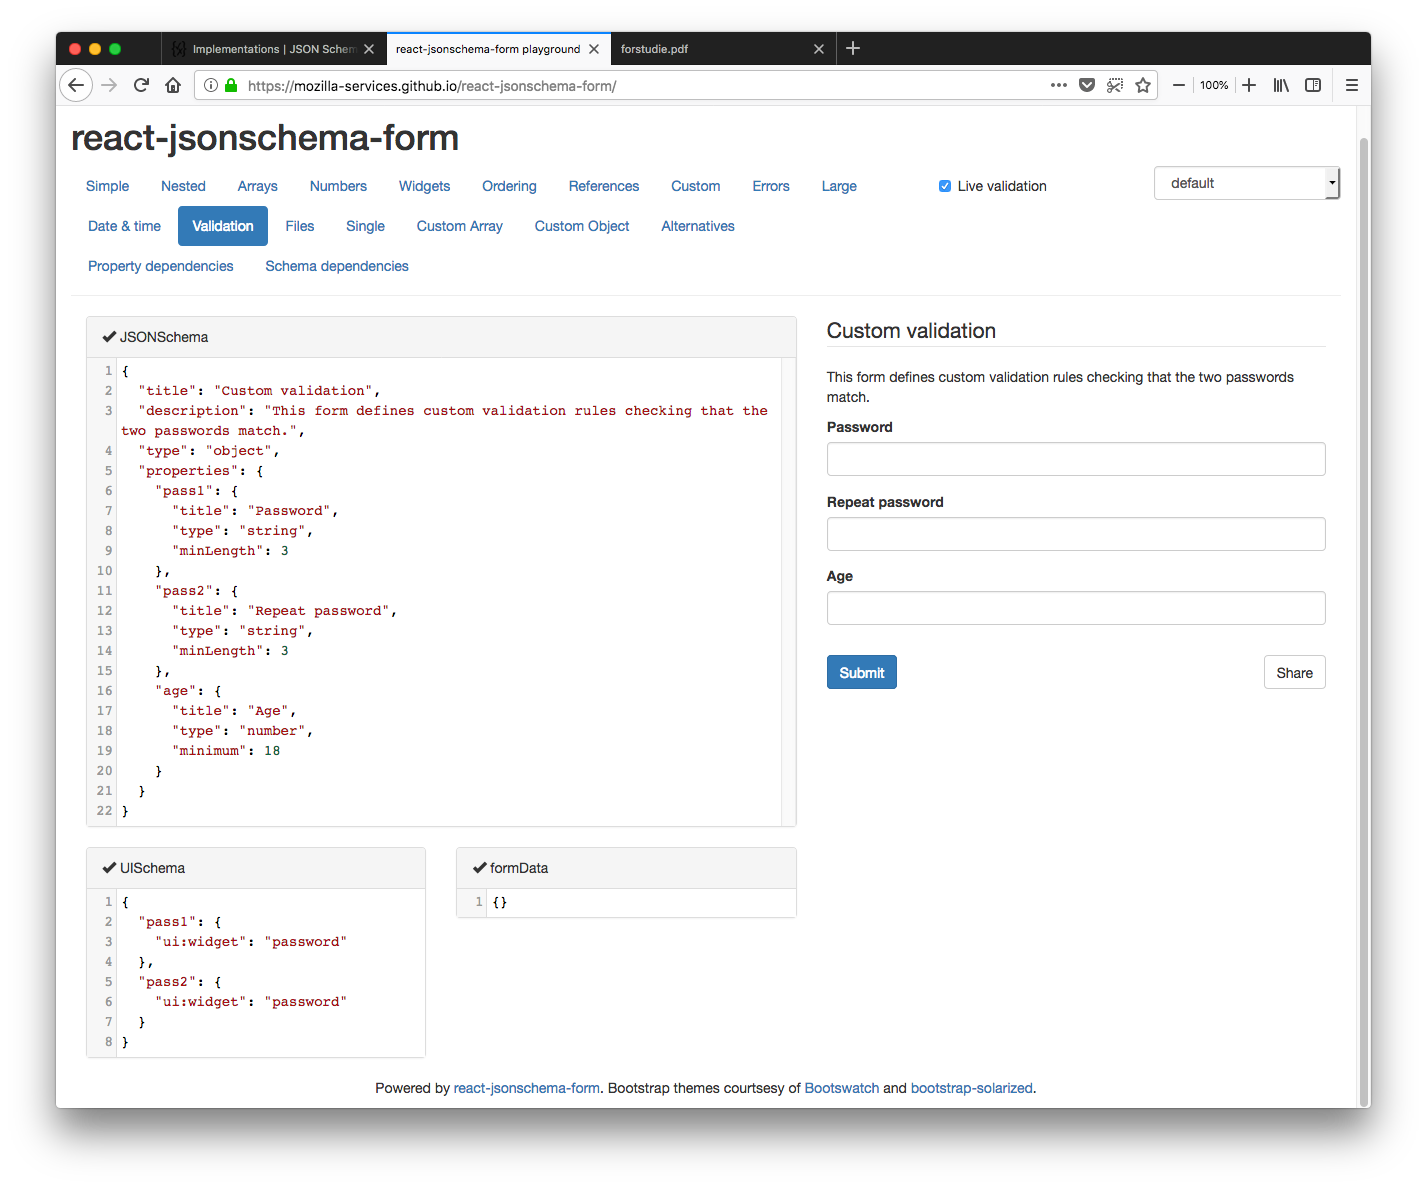
\includegraphics[width=\textwidth]{./images/screenshot-react-jsonschema-form.png}
	\vspace{-1.7em}
	\caption{React JSON Schema Form \cite{MozillaServices}}
	\label{fig:react-jsonschema-form}
\end{figure}

Det som är en nackdel hos \textit{platta formulär} är hur de presenterar djupt komplexa JSON-strukturer. Det är inte uppenbart hur ett grafiskt användargränssnitt skulle visualisera en vektor innehållande objekt med två \textit{properties}, varav ena \textit{propertyn} är ett objekt med två olika vektorer. I ett komplext formulär kan det också vara svårt att veta hur annoteringar som \textit{title} och \textit{description} borde presenteras. För att lösa problemet med representation av komplex data använder verktygen oftast ett externt \textit{``ui-schema''} eller tillägg till JSON Schemat för att tillföra extra annoteringsinformation om formulärets utseende. Det är en riktigt bra kompromiss om lösningen måste kunna klara av att presentera djupt komplexa datatyper, som inte följer en förutbestämd struktur, dock så uppfyller det inte kraven som ställdes på verktygen.

En \textit{trädstruktur} hanterar representation av djupt komplex data som \textit{platta formulär} inte klarar av lika bra. Det kan vara enklare att förstå den övergripande strukturen med en \textit{trädstruktur}, vilket speciellt gynnar datatyperna objekt och vektorer. Däremot bidrar \textit{platta formulär} mycket bättre förklaringar av enstaka datanoder som är någon av de andra datatyperna, vilket ger bättre förståelse för datanoderna, vilket \textit{trädstrukturer} inte lyckas med.